\section{Diskussion}
\label{sec:Diskussion}

\subsection{Reflexionsgesetz}

Messwerte: \autoref{tab:Aufgabe1}\\ \\

Das Reflexionsgesetz besagt, dass der Einfallswinkel genauso groß ist wie der Ausfallswinkel. Also, dass die Differenz der
beiden Winkel $0^{\circ}$ ist.\\
Als Ergebnis unserer Funktionsreihe besteht eine Differenz von $x = 0,2143^{\circ} \pm 0,7071^{\circ}$. Da Null im Fehlerintervall
liegt, gilt das Reflexionsgesetz anhand des Experiments als bewiesen.

\subsection{Brechungsgesetz}

Messwerte: \autoref{tab:Aufgabe2}\\ \\

Durch die Messwertreihe zum Versuch, wird ein Wert von $n = 1,515 \pm 0,035$ für den Brechungsindex von Plexiglas gewonnen. Der
Literaturwert des Brechungsindex' von Plexiglas ist $n = 1,492$. Da dieser Wert im Fehlerintervall liegt und wir nur kleine Meßfehler haben,
lässt sich das Brechungsgesetz nach Snellius hiermit beweisen.

\subsection{Planparallele Platten}

Messwerte: \autoref{tab:Aufgabe4a} , \autoref{tab:Aufgabe4b}\\ \\

Da beide verwendeten Methoden sehr ähnliche Ergebnisse liefern, mit Abweichungen von wenigen Millimetern (Abweichungen von ca. 0,77 \%), lassen sich beide Methoden als
valide identifizieren.\\
Da man bei der zweiten Methode nur einen Satz an Messwerten mit Meßfehlern hat, ist hier die Fehlerfortpflanzung geringer und man erhält genauere
Ergebnisse. Deswegen ist Methode zwei der ersten gegenüber zu bevorzugen.\\
Durch die Verwendung beider Methoden, lassen sich zudem die Ergebnisse der vorangegangenen Versuche verifizieren.

\subsection{Prisma}

Messwerte: \autoref{tab:Aufgabe5a1} , \autoref{tab:Aufgabe5a2} , \autoref{tab:Aufgabe5b1} , \autoref{tab:Aufgabe5b2}\\ \\

Die Ablenkung $\delta$ sollte antiproportional zu Wellenlänge anwachsen. Je größer die Wellenlänge des Lichts, desto kleiner ist
die Ablenkung des Lichts. Da rotes Licht eine größere Wellelänge hat als grünes Licht, sollte hier die Ablenkung kleiner sein.\\
Die Ablenkung des roten Lichtstrahls betrug $\delta = 39,6 \pm 0,4 ^{\circ}$ und des Grünen $\delta = 40,1 \pm 0,4 ^{\circ}$. Da der grüne
Laser tatsächlich stärker abgelenkt wurde, kann diese Gesetzmäßigkeit ebenfalls als bestätigt angesehen werden.

\subsection{Beugung am Gitter}

Messwerte: \autoref{tab:Aufgabe6a} , \autoref{tab:Aufgabe6b} , \autoref{tab:Aufgabe6c} \\ \\

Die Messwerte zeigen zu den Literaturwerten Abweichungen nach unten zwischen 28,35 \% und 34,4 \%. Das sind sehr hohe Abweichungen 
und deuten auf einen systematischen Fehler hin. Meßungenauigkeiten kommen hier wahrscheinlich dadurch zustande, dass die Winkelskala per
Hand justiert werden musste und öfters verrutscht ist, wodurch falsche Winkel abgelesen werden.\\
Zudem kann ein genereller Fehler beim Versuchsaufbau untergekommen sein. Die Versuchsapparatur könnte ebenfalls defekt gewesen sein.\\
Durch diesen Versuch ließ sich die Gesetzmäßigkeit zur Beugung am Gitter leider nicht beweisen.

\section{Messwerte}
\label{sec:Messwerte}

\begin{figure}
  \centering
  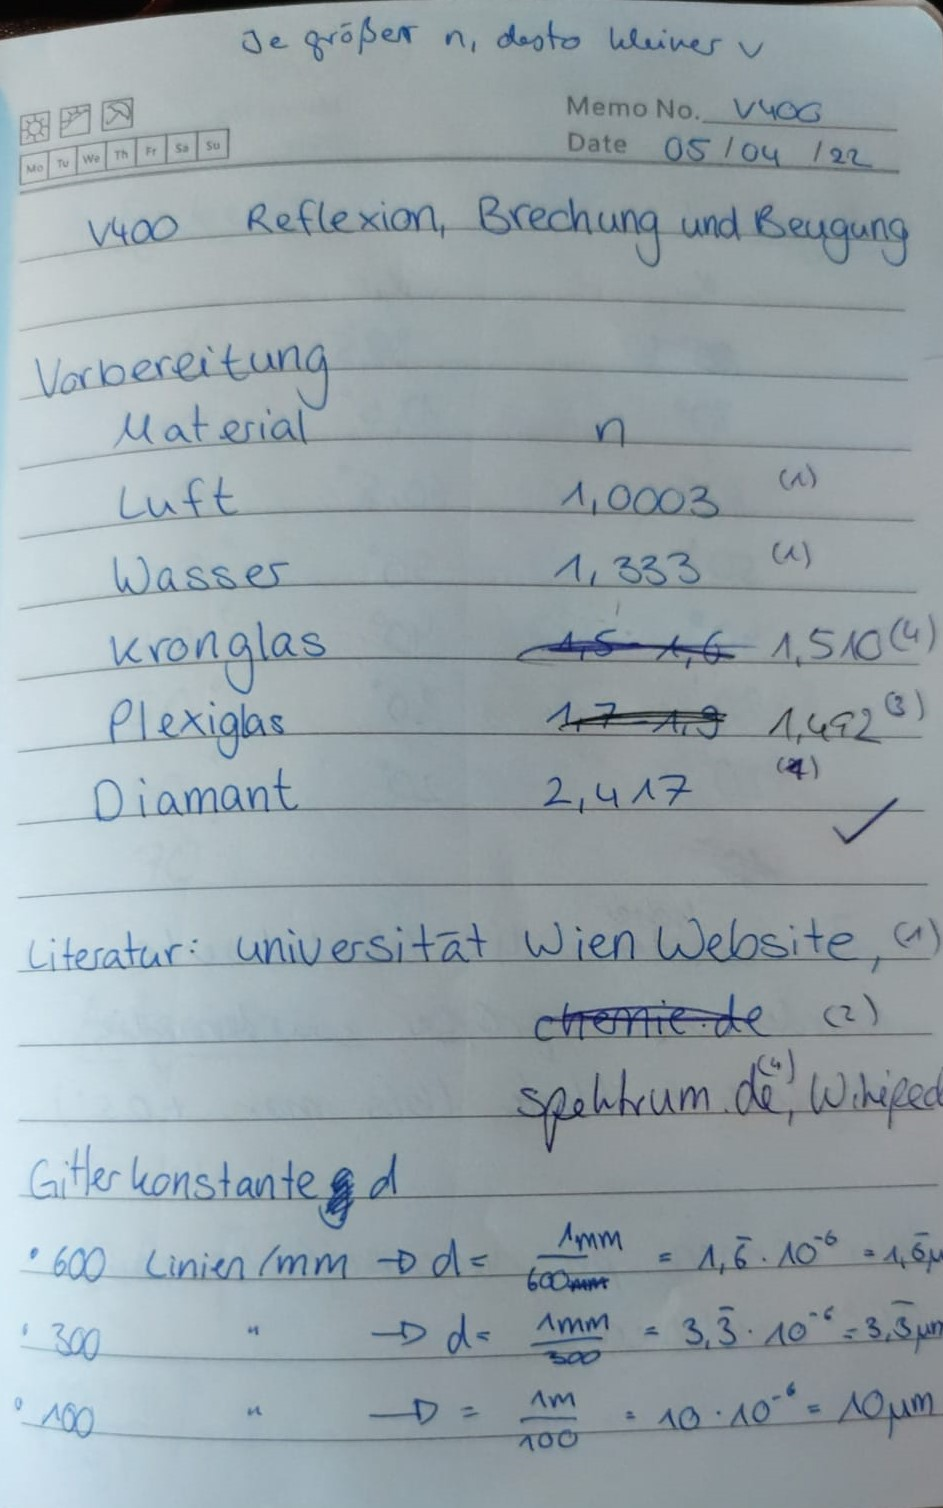
\includegraphics[width=0.7\textwidth]{Messwerte/Vorbereitungsaufgabe.jpeg}
  \caption{Vorbereitungsaufgabe.}
  \label{fig:M1}
\end{figure}

\begin{figure}
  \centering
  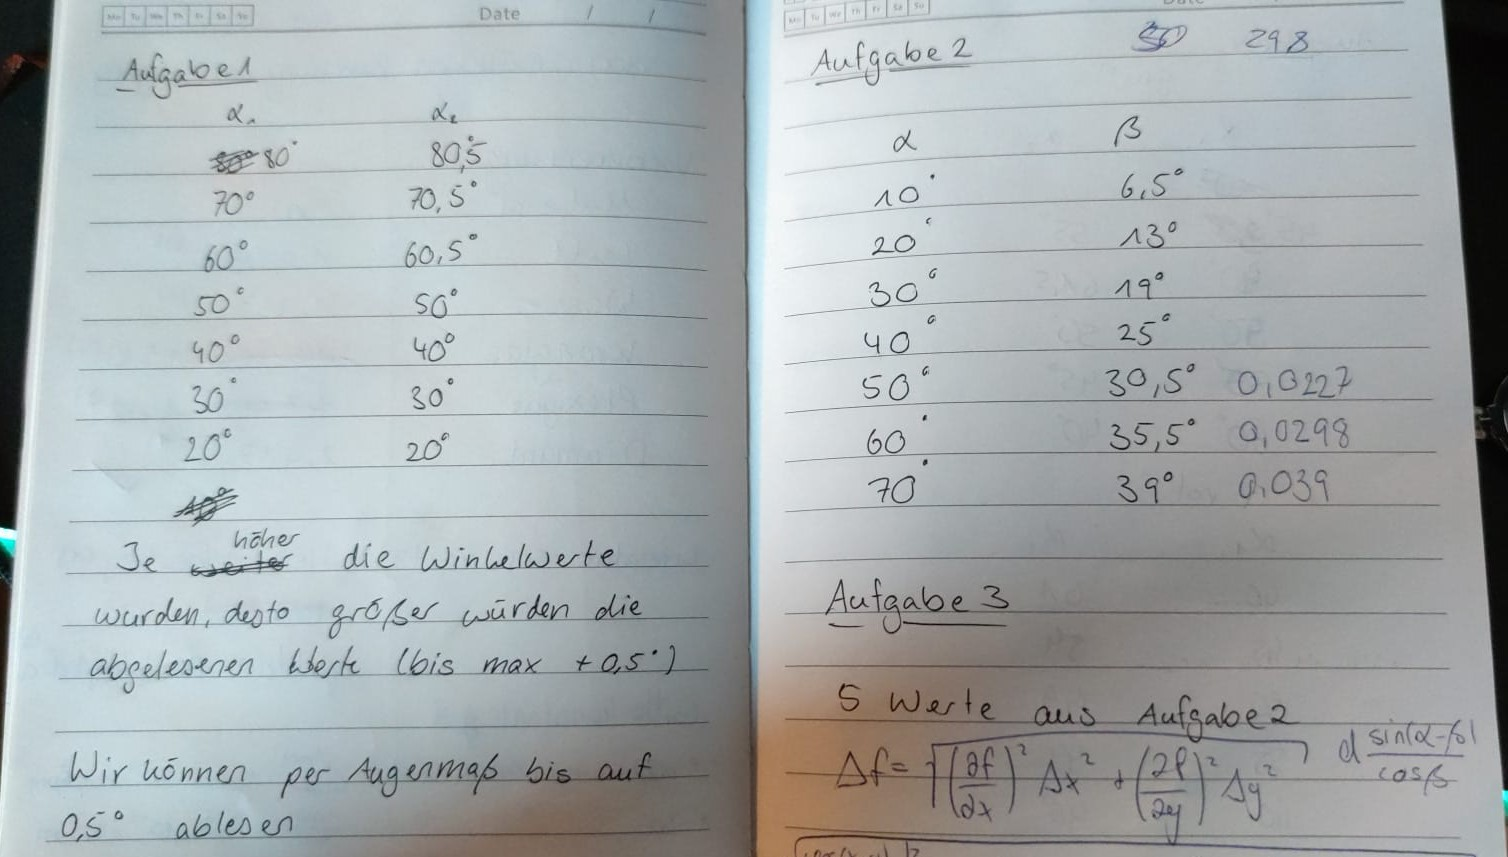
\includegraphics[width=0.7\textwidth]{Messwerte/Aufgabe1,2,3.jpeg}
  \caption{Aufgabe 1, 2, 3.}
  \label{fig:M2}
\end{figure}

\begin{figure}
  \centering
  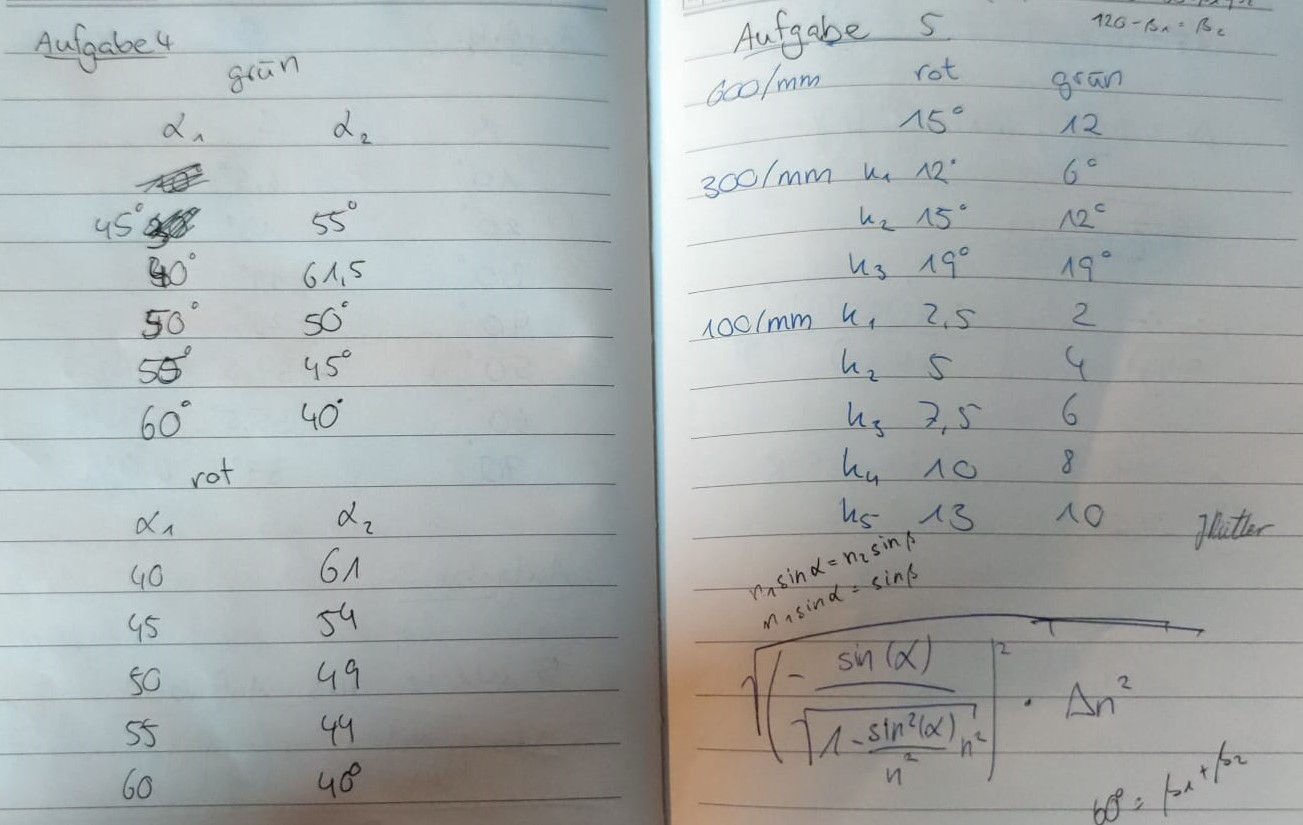
\includegraphics[width=0.7\textwidth]{Messwerte/Aufgabe4,5.jpeg}
  \caption{Aufgabe 4, 5}
  \label{fig:M3}
\end{figure}